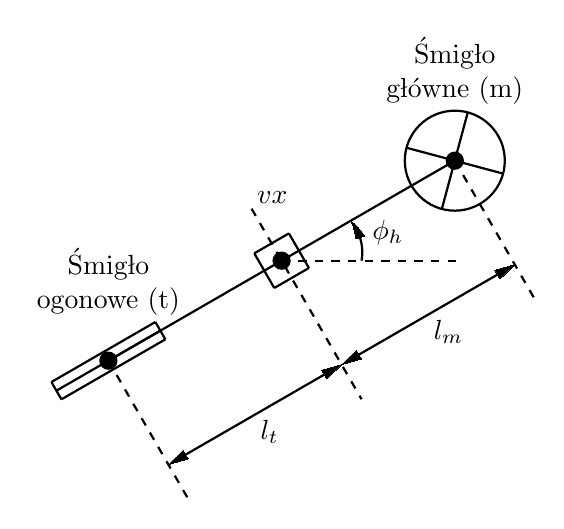
\begin{tikzpicture}[scale=2.54]
% dpic version 2015.10.28 option -g for TikZ and PGF 1.01
\ifx\dpiclw\undefined\newdimen\dpiclw\fi
\global\def\dpicdraw{\draw[line width=\dpiclw]}
\global\def\dpicstop{;}
\dpiclw=0.8bp
\dpicdraw (0.025021,-0.149998)
 --(0.050022,-0.193299)\dpicstop
\dpicdraw (0.050022,-0.193299)
 --(0.309832,-0.043303)\dpicstop
\dpicdraw (0.309832,-0.043303)
 --(0.569642,0.106693)\dpicstop
\dpicdraw (0.569642,0.106693)
 --(0.544645,0.149996)\dpicstop
\dpicdraw (0.544645,0.149996)
 --(0.519648,0.193299)\dpicstop
\dpicdraw (0.519648,0.193299)
 --(0.259824,0.043327)\dpicstop
\dpicdraw (0.259824,0.043327)
 --(0,-0.106645)\dpicstop
\dpicdraw (0,-0.106645)
 --(0.025001,-0.149946)\dpicstop
\dpicdraw[fill=black](0.284828,0.000012) circle (0.015748in)\dpicstop
\dpicdraw (0.025021,-0.149998)
 --(0.544645,0.149996)\dpicstop
\dpicdraw (0.284821,0)
 --(1.150854,0.499987)\dpicstop
\dpicdraw[fill=black](1.150854,0.499987) circle (0.015748in)\dpicstop
\dpicdraw (1.150854,0.499987)
 --(2.016887,0.999973)\dpicstop
\dpicdraw (2.016887,0.999973) circle (0.098425in)\dpicstop
\dpicdraw (2.081601,1.241452)
 --(1.952151,0.7585)\dpicstop
\dpicdraw (2.258369,0.93527)
 --(1.775399,1.064654)\dpicstop
\dpicdraw[fill=black](2.016887,0.999973) circle (0.015748in)\dpicstop
\dpicdraw[dashed](1.150854,0.499987)
 --(2.050854,0.499987)\dpicstop
\filldraw[line width=0bp](1.543124,0.616532)
 --(1.520912,0.609517)
 ..controls (1.51879,0.640891) and (1.510768,0.671582)
 ..(1.497268,0.699981)
 ..controls (1.524985,0.67947) and (1.54816,0.653447)
 ..(1.565335,0.623548)
 --(1.543124,0.616532)\dpicstop
\dpicdraw[line width=0.8bp](1.522866,0.662374)
 ..controls (1.550279,0.612963) and (1.560144,0.555723)
 ..(1.550854,0.499987)\dpicstop
\draw (1.682115,0.642333) node{$\phi_h$};
\dpicdraw (1.064248,0.449983)
 --(1.11425,0.363382)\dpicstop
\dpicdraw (1.11425,0.363382)
 --(1.200854,0.413381)\dpicstop
\dpicdraw (1.200854,0.413381)
 --(1.287457,0.46338)\dpicstop
\dpicdraw (1.287457,0.46338)
 --(1.237462,0.549985)\dpicstop
\dpicdraw (1.237462,0.549985)
 --(1.187468,0.636591)\dpicstop
\dpicdraw (1.187468,0.636591)
 --(1.10086,0.5866)\dpicstop
\dpicdraw (1.10086,0.5866)
 --(1.014252,0.53661)\dpicstop
\dpicdraw (1.014252,0.53661)
 --(1.064254,0.450009)\dpicstop
\draw (0.284821,0.393299) node{\shortstack{Śmigło\\%
ogonowe (t)}};
\draw (2.016887,1.449973) node{\shortstack{Śmigło\\%
główne (m)}};
\dpicdraw[dashed](1.00087,0.759804)
 --(1.550876,-0.192821)\dpicstop
\dpicdraw[dashed](0.284821,0)
 --(0.684843,-0.692808)\dpicstop
\dpicdraw[dashed](2.016887,0.999973)
 --(2.416909,0.307165)\dpicstop
\draw (1.00087,0.759804) node[above right=-1.5bp]{$vx$};
\filldraw[line width=0bp](1.376767,-0.091269)
 --(1.45087,-0.019619)
 --(1.351767,-0.047967) --cycle\dpicstop
\filldraw[line width=0bp](0.658941,-0.447956)
 --(0.584837,-0.519606)
 --(0.68394,-0.491258) --cycle\dpicstop
\dpicdraw (1.431033,-0.031072)
 --(0.604675,-0.508153)\dpicstop
\draw (1.017854,-0.269613) node[below right=-1.5bp]{$l_t$};
\filldraw[line width=0bp](1.524974,0.05203)
 --(1.45087,-0.019619)
 --(1.549973,0.008728) --cycle\dpicstop
\filldraw[line width=0bp](2.2428,0.408718)
 --(2.316903,0.480367)
 --(2.2178,0.452019) --cycle\dpicstop
\dpicdraw (1.470708,-0.008167)
 --(2.297066,0.468915)\dpicstop
\draw (1.883887,0.230374) node[below right=-1.5bp]{$l_m$};
\end{tikzpicture}
